\documentclass[SoftwareDesign/SoftwareDesign_main.tex]{subfiles}

\begin{document}
\section{Design af Header Bar}
Dette afsnit præsenterer designet af et View og en ViewModel til det, der er headerbaren. Der er valgt en tilgang til designet, der hedder ViewFirst, hvor Viewet laves først og derudfra laves funktionaliteten i ViewModel, så det stemmer overens med arkitekturen omkring HeaderBaren.
\subsection{Design af View til Header baren}
Til design af Headerbaren tages der udgangspunkt i de WireFrames lavet for applikationen, der ses i figur \ref{fig:headerbar_wf}. 
\begin{figure}[H]
    \centering
    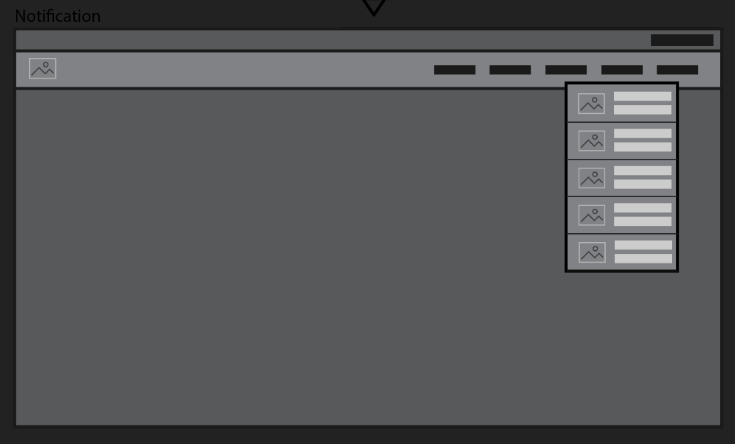
\includegraphics[width=\textwidth]{SoftwareDesign/MVVMDesigns/Graphics/HeaderBarWireFrame.png}
    \caption{Header Bar WireFrame, der tages udgangspunkt i, i design af Viewet}
    \label{fig:headerbar_wf}
\end{figure}
Det der kendetegner HeaderBaren er, at det er en bar i toppen af Applikationen, der går på tværs af applikationen, og kan findes på samtlige sider. Det er også gennem denne, at man som en bruger navigerer gennem applikationen ved brug af navigationsredskaber(knapper, osv). Da man ikke skal være i stand til at navigere fra Login og Usersignup siden, inden man er godkendt som bruger, er dette dog den eneste undtagelse for, hvor headerbaren skal vises.\\

Nu hvor headerbarens funktionalitet er defineret meget overordnet, giver det mening at dykke lidt ned i de enkelte funktionaliteter. Tages der igen udgangspunkt i figur \ref{fig:headerbar_wf}, så ses der i venstre side af baren et billede. Dette billede bør fungere, som navigation tilbage til startsiden, og samtidig vise logoet for applikationen. Det næste, der kan ses i headerbaren er en søgebar, der giver brugeren mulighed for lynhurtigt at søge efter en bil i deres nærområde. Efter søgebaren kommer flere navigationsknapper, der skal tage brugeren til henholdsvis Brugerprofil- og Bilsøgnings-siden. Så er der en notifikationsknap, der skal lave en dropdown-menu med alle notifikationer. Til sidst er der en knap, så brugeren kan logge ud.

\subsection{Design af ViewModel til Header baren}
Meget af funktionaliteten er givet ud fra Viewet og Arkitekturen, hvilket gør den nem at designe. Der skal for alle knapperne, der kun har noget med navigation at gøre, være en kommando, der ved brug af ApplikationsViewModellen går til den rigtige side. Der er nogle enkelte særtilfælde for navigationen, der er til Søgebaren og LogUd.\\

Startes der med Søgebaren, skal den indtastede streng sendes med ved navigationen. Dette kan umiddelbart gøres ved, at have en string, man kan binde til i viewmodellen. Når så søgningen foretages (tryk på søg knappen eller keyboard-enter) så kan man gennem en EventAggregator smide et event til SearchViewModel om at der foretages en søgning  på den ønskede string.\\

Logud derimod skal først sørge for at fjerne brugeren fra applikationen og herefter navigere til LoginViewet.\\

Den næste funktionalitet, der skiller sig ud er notifikationsknappen. Selve det med at vise en popup-menu kan gøres rent i xaml. Da hver notifikationerne og hvert notifikationsitem har deres egen ViewModel, så er det ikke op til headerbaren at tage hånd om dette. HeaderbarViewModel skal dog abonnere på om, der er en ny ulæst notifikation, hvilket igen gøres igennem Event Aggregator.

\end{document}